% ----------------------------------------------------------------------------
% Apresentação
% ----------------------------------------------------------------------------
 
\chapter{Apresentação}

Pure Data é um ambiente visual de programação musical que permite a criação de
aplicações musicais complexas a partir da combinação de componentes visuais
mais simples chamados \textbf{objetos}. As distribuições oficiais do Pure Data
contêm diversos objetos prontos para o uso, mas também permitem a extensão de
suas funcionalidades através da criação de novos objetos utilizando C/C++.
Desta forma, novas linhas de código escritas pelo usuário são compilados como
bibliotecas dinâmicas e podem ser carregadas pelo programa em tempo de
execução. Objetos desta forma levam o nome de \textbf{\\externals}.

Este é um tutorial prático para o desenvolvimento de \externals em C para o
Pure Data. A iniciativa de escrever este documento surgiu no primeiro semestre
de 2011, durante a disciplina de Computação Musical ministrada pelo professor
Marcelo Gomes de Queiroz no Instituto de Matemática e Estatística da
Universidade de São Paulo. A intenção deste tutorial é auxiliar programadores
a desenvolver \externals de maneira bastante simples através de exemplos
práticos.

Mais do que ampliar a gama de objetos do Pure Data e criar novos objetos, o
objetivo deste trabalho é também fornecer ao pesquisador de computação musical
uma ferramenta para implementar e testar algoritmos de processamento de áudio
para caráter de estudo. Isto significa que podemos reimplementar várias coisas
que já existem no Pure Data simplesmente porque é didático programar e colocar
algoritmos para funcionar.

\section{Escrevendo \externals}

O código fonte do Pure Data é organizado de acordo com convenções de
programação orientada a objetos. Para o desenvolvimento de \externals, é
necessário seguir estas convenções e fornecer ao ambiente uma nova classe com
alguns métodos específicos, como veremos mais adiante. Para desenvolver para o
Pure Data, é necessário importar o arquivo de cabeçalho
\texttt{m\_pd.h}\footnote{http://pure-data.git.sourceforge.net/git/gitweb.cgi?p=pure-data/pure-data;a=blob\_plain;f=src/m\_pd.h;hb=HEAD},
que contém definições de constantes, tipos e funções.

Uma boa fonte de informação é o tutorial de
\externals\footnote{http://iem.at/pd/externals-HOWTO/pd-externals-HOWTO.pdf}
escrito pelo IOHannes\footnote{http://puredata.info/author/zmoelnig}, um dos
programadores do Pure Data. Apesar de ter utilizado este documento como ponto
de partida, boa parte do que está incluso no presente tutorial foi aprendido a
partir da leitura do código-fonte de \externals contidos no repositório
oficial do Pure
Data\footnote{http://pure-data.svn.sourceforge.net/viewvc/pure-data/trunk/externals/}.

\section{Organização do código-fonte e do objeto compilado}

Um novo \external corresponde a uma nova classe na arquitetura orientada a
objetos do Pure Data. Para que o carregamento da biblioteca dinâmica
em tempo de execução funcione corretamente, é necessário que o
arquivo binário produzido possua o mesmo nome que a classe correspondente ao
\external.

Para criar, por exemplo, um \external chamado ``passa-baixas", podemos
escrever seu código-fonte em um arquivo chamado \texttt{passa-baixas.c}, e em
seguida compilar um objeto de biblioteca compartilhada chamado
\texttt{passa-baixas.pd\_linux}, no caso do sistema GNU/Linux. Outras
arquiteturas de sistema utilizam outras extensões para o nome do objeto com a
biblioteca compartilhada do \external, como por exemplo \texttt{.dll} (M\$
Windows), \texttt{.pd\_irix5} (SGI Irix) ou \texttt{.pd\_darwin} (Mac OS X).

\textbf{Importante:} O nome do arquivo com o código-fonte não possui formato
obrigatório, mas o nome do objeto compilado com a biblioteca dinâmica deve
sempre corresponder ao nome da classe, assim como sua extensão deve sempre
corresponder à arquitetura do sistema utilizado.

\section{Compilação}

Um \external precisa ser primeiro compilado e em seguida transformado em
objeto compartilhado, para poder ser carregado em tempo de execução pelo Pure
Data. A versão Linux pode ser feita com os comandos:

\vspace{1em}
\begin{lstlisting}
EXTNAME=meu-external
cc -DPD -fPIC -Wall -o ${EXTNAME}.o -c ${EXTNAME}.c
ld -shared -lc -lm -o ${EXTNAME}.pd_linux ${EXTNAME}.o
rm example1.o
\end{lstlisting}

Para facilitar a compilação, o ideal é utilizar um \texttt{makefile}. Os
exemplos deste tutorial estão acompanhadas de um \texttt{makefile} produzido
pelo professor Marcelo Queiroz, adaptado para esta ocasião.

\section{Arquivos de ajuda}

Como convenção, o arquivo de ajuda deve ter o mesmo nome que o \external. Por
exemplo, para o código fonte \texttt{example01.c}, que gera o objeto
\texttt{example01.pd\_linux}, escrevemos também o arquivo
\texttt{example01-help.pd}. Este arquivo do Pure Data com exemplos deve
acompanhar o \external na instalação, residindo na mesma pasta que objeto
compilado com a biblioteca compartilhada.  Há também a possibilidade de
associação de outros arquivos que não sigam esta convenção a um \external.
Esta possibilidade será apresentada no próximo capítulo.

\section{Utilizando \externals}

Para carregar um \external em um \texttt{patch} do Pure Data em tempo de
execução, basta criar um objeto (com \texttt{CTRL+1} ou acessando o menu
\texttt{Put} $\rightarrow$ \texttt{Object}) com o caminho (relativo ou
absoluto) para o objeto compilado com a biblioteca compartilhada, omitindo a
extensão.

É possível adicionar o diretório que contém o arquivo binário do \external ao
caminho de busca do Pure Data, de forma que para acessá-lo de dentro de um
\patch não seja necessário digitar o caminho inteiro até o objeto. Isto pode
ser feito através da passagem de um parâmetro na linha de comando do Pure Data
com a opção \texttt{-path <caminho>}, ou de forma gráfica acessando a opção
\texttt{File} $\rightarrow$ \texttt{Path...} no menu do Pure Data,
como pode ser visto na figura \ref{fig:search-path}.

\begin{figure}[h!]
  \centering
  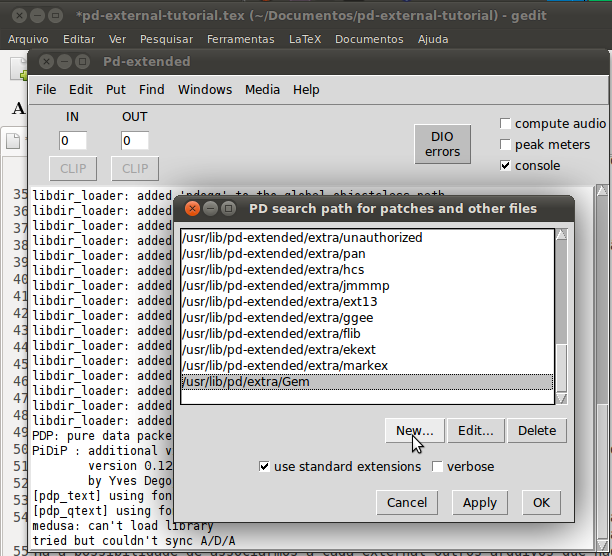
\includegraphics[width=0.7\textwidth]{path}
  \caption{Adicionando o diretório de um \external ao caminho de busca do Pure Data.}
  \label{fig:search-path}
\end{figure}

Para carregar uma biblioteca de \externals (mais de um \external no mesmo
arquivo-fonte), é possível indicar o nome da bibliotecai na linha
de comando do Pure Data utilizando a opção \texttt{-lib <biblioteca>}, ou
também graficamente através do menu \texttt{File} $\rightarrow$
\texttt{Startup...}, como pode ser visto na figura \ref{fig:lib}.

\begin{figure}[h!]
  \centering
  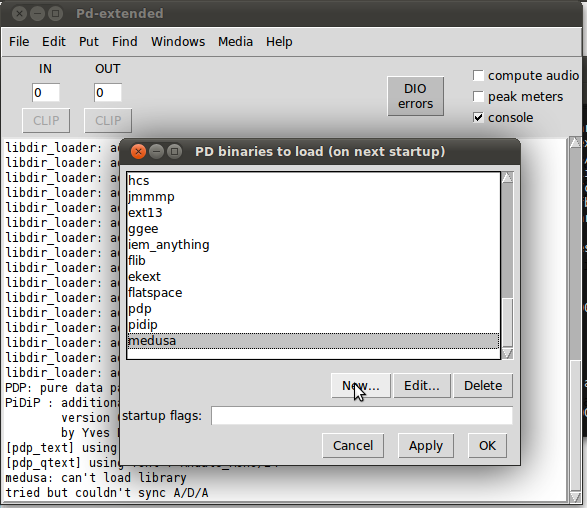
\includegraphics[width=0.7\textwidth]{startup}
  \caption{Adicionando uma biblioteca ao Pure Data.}
  \label{fig:lib}
\end{figure}

